\section{eo\-Second\-Moment\-Stats$<$ EOT $>$ Class Template Reference}
\label{classeo_second_moment_stats}\index{eoSecondMomentStats@{eoSecondMomentStats}}
Average fitness + Std.  


{\tt \#include $<$eo\-Stat.h$>$}

Inheritance diagram for eo\-Second\-Moment\-Stats$<$ EOT $>$::\begin{figure}[H]
\begin{center}
\leavevmode
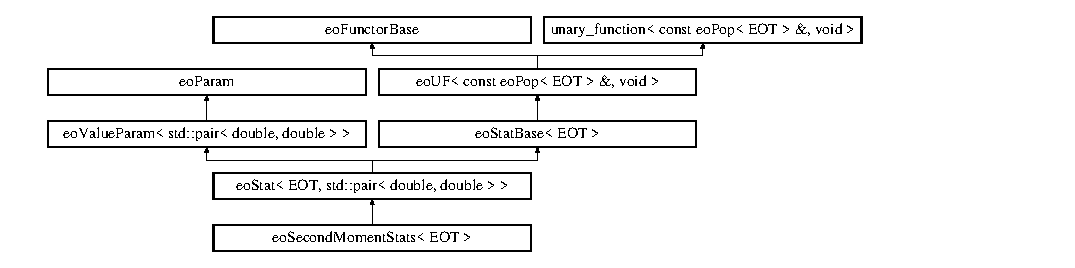
\includegraphics[height=3.15315cm]{classeo_second_moment_stats}
\end{center}
\end{figure}
\subsection*{Public Types}
\begin{CompactItemize}
\item 
typedef EOT::Fitness {\bf fitness\_\-type}\label{classeo_second_moment_stats_w0}

\item 
typedef std::pair$<$ double, double $>$ {\bf Square\-Pair}\label{classeo_second_moment_stats_w1}

\end{CompactItemize}
\subsection*{Public Member Functions}
\begin{CompactItemize}
\item 
{\bf eo\-Second\-Moment\-Stats} (std::string \_\-description=\char`\"{}Average \& Stdev\char`\"{})\label{classeo_second_moment_stats_a0}

\item 
virtual void {\bf operator()} (const {\bf eo\-Pop}$<$ {\bf EOT} $>$ \&\_\-pop)\label{classeo_second_moment_stats_a1}

\begin{CompactList}\small\item\em The pure virtual function that needs to be implemented by the subclass. \item\end{CompactList}\item 
virtual std::string {\bf class\-Name} (void) const \label{classeo_second_moment_stats_a2}

\end{CompactItemize}
\subsection*{Static Public Member Functions}
\begin{CompactItemize}
\item 
Square\-Pair {\bf sum\-Of\-Squares} (Square\-Pair \_\-sq, const {\bf EOT} \&\_\-eo)\label{classeo_second_moment_stats_e0}

\end{CompactItemize}


\subsection{Detailed Description}
\subsubsection*{template$<$class EOT$>$ class eo\-Second\-Moment\-Stats$<$ EOT $>$}

Average fitness + Std. 

dev. of a population, fitness needs to be scalar. 



Definition at line 168 of file eo\-Stat.h.

The documentation for this class was generated from the following file:\begin{CompactItemize}
\item 
eo\-Stat.h\end{CompactItemize}
